%!TEX root = Thesis.tex

\chapter{Clustering: basic concepts, definitions and algorithms}
\label{chapter:clustering}

%this is mostly taken from Jain's 50 years beyond K-Means
Hundreds of methods for data analysis exist.
Many of these methods fall into the realm of machine learning, which is usually divided into 2 major groups: \textit{supervised} and \textit{unsupervised} learning.
% TODO: add some reference for the 2 major groups; optional: explain what learning is
Supervised learning deals with labeled data, i.e. data for which ground truth is known, and tries to solve the problem of classification.
Examples of supervised learning algorithms are Neural Networks, Decision Trees, Linear Regression and Support Vector Machines. %TODO add refs
 %TODO: add ref for solving classification
Unsupervised learning deals with unlabeled data for which no extra information is known.
An example of algorithms within this paradigm is clustering algorithms, which are the focus of this chapter.
%Clustering algorithms an are example of unsupervised algorithms. % TODO: add refs

This chapter will serve as an introduction to clustering.
It starts by defining the problem of clustering in section \ref{sec:clustering}, goes on to provide useful definitions and notation in section \ref{sec:definitions and notation} and briefly addresses different properties of clustering algorithms in section \ref{sec:clustering properties}.
Two very well known algorithms are presented: K-Means in section \ref{sec:kmeans} and Single-Link in section \ref{sec:sl}.
Evidence Accumulation Clustering is a state of the art ensemble clustering algorithm and the focus of this dissertation.
Section \ref{sec:ensemble} will explain briefly the concept of ensemble clustering followed by an overview and application examples of the EAC algorithm in section \ref{sec:eac}.

\section{The problem of clustering}
\label{sec:clustering}

% have to say that I'm using a vectorial representation of the data (data as vector of features) without loss of generality. I have to specify that I'm dealing with a partitioning clustering but other kinds exist. In this context (of vectorial data and partitional algorithms) K-Means is one of the most known algorithms. It is simple and fast and, although it only yields good results in a specific set of cases, it is often used as a starting point for more robust algorithms, e.g. EAC. 

Cluster analysis methods are unsupervised and the backbone of the present work.
The goal of data clustering, as defined by \cite{Jain2010}, is the discovery of the \textit{natural grouping(s)} of a set of patterns, points or objects.
In other words, the goal of data clustering is to discover structure on data.
The methodology used is to group patterns (usually represented as a vector of measurements or a point in space \cite{Jain1999}) based on some similarity, such that patterns belonging to the same cluster are typically more similar to each other than to patterns of other clusters.
Clustering is a strictly data-driven method, in contrast with classification techniques which have a training set with the desired labels for a limited collection of patterns.
Because there is very little information, as few assumptions as possible should be made about the structure of the data (e.g. number of clusters).
And, because clustering typically makes as few assumptions on the data as possible, it is appropriate to use it on exploratory structural analysis of the data.
The process of clustering data has three main stages \cite{Jain1999}:

\begin{itemize}
    \item \textbf{Pattern representation} refers to the choice of representation of the input data in terms of size, scale and type of features.
    The input patterns may be fed directly to the algorithms or undergo \emph{feature selection} and/or \emph{feature extraction}. The former is simply the selection of which features of the originally available should be used.
    The latter deals with the transformation of the original features such that the resulting features will produce more accurate and insightful clusterings, e.g. Principal Component Analysis.
    % It should be noted that

    \item \textbf{Pattern similarity} refers to the definition of a measure for computing the similarity between two patterns.
    \item \textbf{Grouping} refers to the algorithm that will perform the actual clustering on the dataset with the defined pattern representation, using the appropriate similarity measure.
\end{itemize}

%TODO iris dataset reference
As an example, Figure \ref{fig:intro raw} shows the plot of the Iris data set \cite{anderson1936species,fisher1936use}, a small well-known Machine Learning data set.
This data set has 4 features, of which only 2 are represented, and 3 classes, of which 2 are overlapping.
A class is overlapping another if they share part of the feature space, i.e. there is a zone in the feature space whose patterns might belong to either class.
Figure \ref{fig:intro natural} presents the desired clustering for this data set.

% Part of this went to the K-Means section
% The number of clusters was purposefully set to an "incorrect" number to demonstrate that the number of cluster of a dataset is not trivial to discover, even in such a simple example.
% In this synthetic dataset, the number of clusters is not clear due to the two superimposed Gaussians.
% The number of clusters is a common initialization parameter for clustering methods.
% When no prior information about the dataset is given, the number of clusters can be hard to discover.

\begin{figure}[!ht]
    \centering
    \begin{subfigure}[b]{0.45\textwidth}
        \centering
        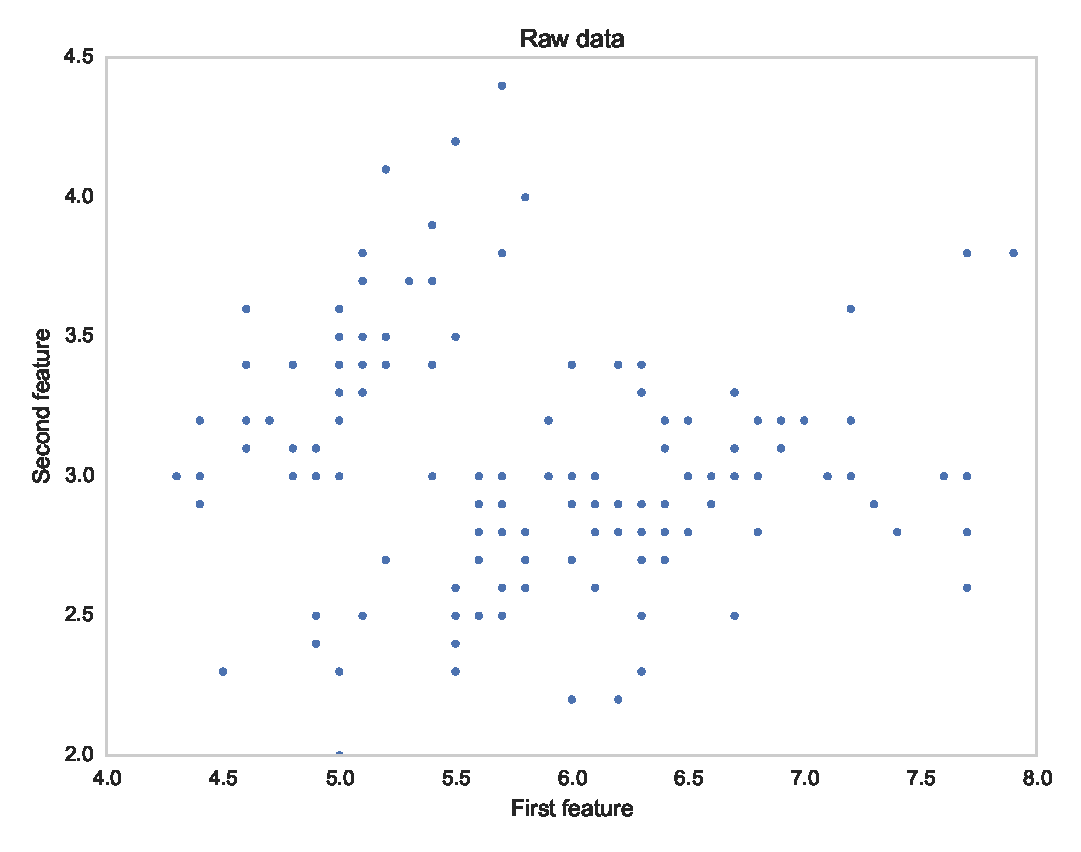
\includegraphics[width=\textwidth]{clustering/raw_data}
        \caption{Input data, unlabeled.}
        \label{fig:intro raw}
    \end{subfigure}
    %\hfill
    \begin{subfigure}[b]{0.45\textwidth}
        \centering
        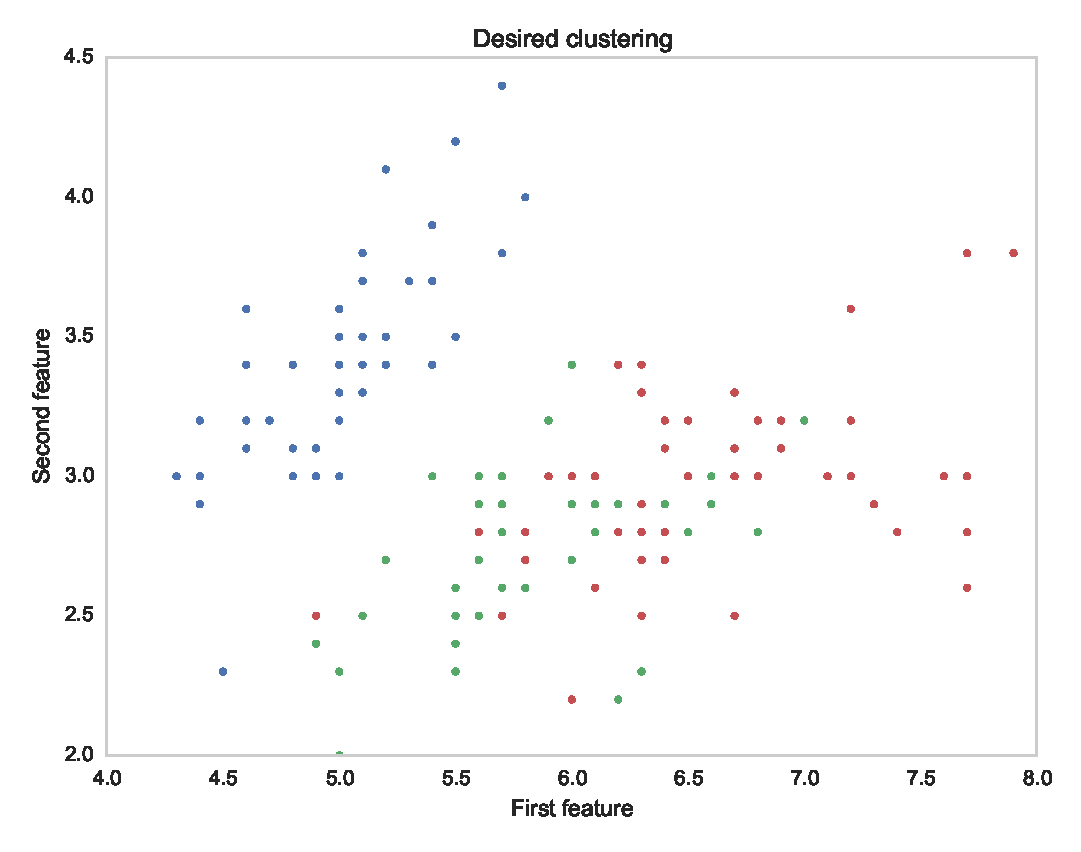
\includegraphics[width=\textwidth]{clustering/desired}
        \caption{Desired labels.}
        \label{fig:intro natural}
    \end{subfigure}

    \caption{First and second features of the Iris dataset. Fig. \ref{fig:intro raw} shows the raw input data, i.e. how the algorithms "see" the data. Fig. \ref{fig:intro natural} shows the desired labels for each point, where each color is coded to a class.}
    \label{fig:clustering plots}
\end{figure}


\section{Definitions and Notation}
\label{sec:definitions and notation}

This section will introduce relevant definitions and notation within the clustering context that will be used throughout the rest of this document and were largely adopted from \cite{Jain1999}.

% TODO: review this part of the vector notation, it is fishy right now
%pattern, features
A \emph{pattern} $\mathbf{x}$ is a single data item and, without loss of generality, can be represented as a vector of $d$ \emph{features} $x_i$ that characterize that data item, $\mathbf{x} = (x_1, \ldots, x_d)$, where $d$ is referred to as the dimensionality of the pattern.
%pattern set
A \emph{pattern set} (or data set) $\mathcal{X}$ is then the collection of all $n$ patterns $\mathcal{X} = \{ \mathbf{x}_1, \ldots, \mathbf{x}_n \}$.
The number of features is usually the same for all patterns in a given pattern set.

%classes
In cluster analysis, the desired clustering, typically, is one that reflects the natural structure of the data, i.e. the original ground truth labeling.
In other words, one wants to group the patterns that came from the same state of nature when they were generated, the same \emph{class}.
A class, then, can be viewed as a source of patterns and the effort of the clustering algorithm is to group patterns from the same source.
Throughout this work, these classes will also be referred to as the "natural" or "true" clusterings.
%labels
\emph{Hard} clustering (or partitional) techniques assign a class label $l_i$ to each pattern $\mathbf{x}_i$.
The whole set of labels corresponding to a pattern set $\mathcal{X}$ is given by $\mathcal{L} = \{ l_1, \ldots, l_n \}$, where $l_i$ is the label of pattern $\mathbf{x}_i$.
%partition
% Throughout this document, the whole set of labels may also be referred to as a partition.
Closely related to the whole set of labels is the concept of a \emph{partition}, which completely describes a clustering.
A partition $P$ is a collection of $k$ \emph{clusters}.
A cluster $C$ is a subset of $nc$ patterns $\mathbf{x}_i$ taken from the pattern set, where the patterns belonging to one subset do not belong to any other in the same partition.
A clustering \emph{ensemble} $\mathbb{P}$ is a set $N$ partitions $P^j$ from a given pattern set, each of which is composed by a set of $k_j$ clusters $C^j_i$, where $j=1, \ldots, N$, $i=1, \ldots, k_j$.
Each cluster is composed by a set of $nc^j_i$ patterns that does not intercept any other cluster of the same partition.
The relationship between the above concepts is condensed in the following expressions:

\begin{align*}
    ensemble \qquad & \mathbb{P} = \left \{   P^1, P^2, \ldots P^N   \right \}  \\
    partition \qquad & P^j = \left \{   C^j_1, C^j_2, \ldots C^{j}_{k_j}   \right \}  \\
    cluster \qquad & C^j_i = \left \{   x_1, x_2, \ldots x_{nc^j_i}   \right \}
\end{align*}



%TODO do this part better
%similarity
% Em relação aos conceitos: Proximidade não tem que ser métrica e pode ser semelhança ou dissemelhança. Pode sempre converter-se semelhança em dissemelhança e vice-versa, no entanto o mesmo já não acontece quando se convertem métricas. Uma distância é uma dissemelhança que é uma métrica (obedece às várias propriedades de métrica: simetria; d(x,x)=0 e desigualdade triangular). Quando se faz a conversão de uma distância para uma semelhança pode deixar de ser métrica. Mas isso só é mesmo importante quando se está a usar explicita ou implicitamente no processamento (por exemplo procura de vizinhos mais próximos, etc) a característica de desigualdade triangular. Em geral a propriedade de simetria é suficiente (e que d(x,x)=0 e sim(x,x)>sim(x,y)).

Typically, a clustering algorithm will use a \emph{proximity} measure for determining how alike are two patterns.
A proximity measure can either be a \emph{similarity} or a \emph{dissimilarity} measure.
One can easily be converted to the other and the main difference is that the former increases in value as patterns are more alike, while the latter decreases in value.
A \emph{distance} is a dissimilarity function \emph{d} which yields non-negative real values and is also a \emph{metric}, which means it obeys the following three properties:



\begin{align*} 
    identity \qquad & d(\mathbf{x}_i, \mathbf{x}_i) = 0  \\
    symmetry \qquad & d(\mathbf{x}_i, \mathbf{x}_j) = d(\mathbf{x}_j, \mathbf{x}_i), i \neq j \\ 
    triangle \; inequality \qquad & d(\mathbf{x}_i, \mathbf{x}_j) + d(\mathbf{x}_j, \mathbf{x}_z)  \ge d(\mathbf{x}_x, \mathbf{x}_z)
\end{align*}



% \begin{align}
%     identity \qquad & d(\mathbf{x}_i, \mathbf{x}_i) = 0  \label{eq:identity} \\
%     symmetry \qquad & d(\mathbf{x}_i, \mathbf{x}_j) = d(\mathbf{x}_j, \mathbf{x}_i), i \neq j   \label{eq:symmetry} \\
%     triangle \; inequality \qquad & d(\mathbf{x}_i, \mathbf{x}_j) + d(\mathbf{x}_j, \mathbf{x}_z) \ge d(\mathbf{x}_x, \mathbf{x}_z) \label{eq:triangle inequality}
% \end{align}

where $\mathbf{x}_i$, $\mathbf{x}_j$ and $\mathbf{x}_z$ are 3 unique patterns belonging to the pattern set $\mathcal{X}$.
Examples of proximity measures include the Euclidean distance, the Pearson’s correlation coefficien and Mutual Shared Neighbors \cite{jarvis1973clustering}.
It should be noted that different proximity measures may be more appropriate in different contexts, such as document, biological or time-series clustering.
Furthermore, data can come in different types such as numerical (discrete or continuous) or categorical (binary or multinomial) attributes.
The researcher should take these factors into account as different proximity measures are more appropriate for some type or even heterogeneous type data. 

An introduction of clustering would be incomplete without a discussion on how good is a partition after clustering.
Several \emph{validation measures} exist and they can placed in two main categories \cite{Aggarwal2014}.
\emph{External} measures use \emph{a priori} information about the data to evaluate the clustering against some external structure.
An application of an external measure could be to test how accurate a clustering algorithm is for a particular dataset by matching the output partition against the ground truth.
Examples of such measures include the \emph{Consistency Index} \cite{Fred2001} and a measure of accuracy based on the problem of minimum weighted bipartite graphs matching \cite{lange2004stability}, which throughout the remainder of the present work will be refered to as \emph{H-index}.
\emph{Internal} measures, on the other hand, determine the quality of the clustering without the use of external information about the data.
The Davies-Bouldin index \cite{davies1979cluster} is such a measure.



\section{Characteristics of clustering techniques}
\label{sec:clustering properties}

Clustering algorithms may be categorized and described according to different properties.
For the sake of completeness, a brief discussion of some of their properties will be layed out in this section.

% hierarchical and partitional
%\emph{Partitional} and \emph{hierarchical} algorithms are the two most studied kinds of algorithms \cite{Aggarwal2014}.
It is common to organize cluster algorithms into two distinct types: \emph{partitional} and \emph{hierarchical}.
A partitional algorithm, such as K-Means, is a hard clustering algorithm that will output a partiton where each pattern belongs exclusively to one cluster.
A hierarchical algorithm produces a tree-based data structure called \emph{dendrogram}.
A dendrogram contains different partitions at different levels of the tree which means that the user can easily change the desired number of clusters by simply traversing the different levels.
This is an advantage over a partitional algorithm since a user can analyze different partitions with different numbers of clusters without having to rerun the algorithm.
% agglomerative vs divisive
Hierarchical algorithms can be further split into two approaches: bottom-up (or \emph{agglomerative}) and top-down (or \emph{divisive}).
% agglomerative
The former starts with all patterns as distinct clusters and will group them together according to some dissimilarity measure, building the dendrogram from the ground up; examples of algorithms that take this approach are Single-Link and Average-Link.
%divisive
The latter will start will all patterns in the same cluster and continuosly split it until all patterns are separated, building the dendrogram from the top level to the bottom; this approach is taken by the Principal Directon Divisive Partitioning\cite{Boley1998} and Bisecting K-Means \cite{Steinbach2000} algorithms.


% monothetic vs polithetic
Another characteristic relates to how algorithms use the features for computing similarities.
If all features are used simultaniously the algorithm is called \emph{polithetic}, e.g. K-Means.
Otherwise, if the features are used sequentially, it is called \emph{monothetic}, e.g. \cite{Chavent1998}.

% fuzzy clustering
Contrasting \emph{hard} clustering algorithm are the \emph{fuzzy} algorithms.
A fuzzy algorithm will attribute to each pattern a degree of membership to each cluster.
A partition can still be extracted from this output by choosing, for each pattern, the cluster with higher degree of membership.
An example of a fuzzy algorithm is the Fuzzy C-Means \cite{Bezdek1984}.

% stochastic vs deterministic
Another characteristic is an algorithm's stochasticity.
A \emph{stochastic} algorithms uses a probabilistic process at some point in the algorithms, possibly yielding different results in each run, e.g. K-Means can use a random initialization.
As an example, the K-Means algorithm typically picks the initialization centroids randomly.
A \emph{deterministic} algorithm, on the other hand, will always produce the same result for a given input, e.g. Single-Link.

Finally, the last characteristic discussed is how an algorithm processes the input data.
An algorithm is said to be \emph{incremental} if it processes the input incrementally, i.e. taking part of the data, processing it and then doing the same for the remaining parts, e.g. PEGASUS \cite{Kang2011}.
A \emph{non-incremental} algorithm, on the other hand, will process the whole input in each run, e.g. K-Means.
This discussion is specially relevant when considering large datasets that may not fit in memory or whose processing would take too long for a single run and is therefore done in parallel.



% % examples of cluster analysis
% Cluster analysis is a relevant technique across several domains (\cite{Aggarwal2014}):

% \begin{itemize}
% 	\item grouping users with similar behaviour or preferences in \textbf{customer segmentation};
% 	\item image segmentation in the field of \textbf{image processing};
% 	\item clustering gene expression data, among other application, in the domain of \textbf{biological data analysis};
% 	\item generation of hierarchical structure for easy access and retrieval of \textbf{information systems}; % not referenced in book
% \end{itemize}

% Clustering is used in a wide variety of fields to solve numerous problems, e.g.:
% %TODO provide references to all of this
% % see https://sites.google.com/site/dataclusteringalgorithms/clustering-algorithm-applications
% % has applications with articles
% \begin{itemize}
% \item image segmentation in the field of image processing;
% \item generation of hierarchical structure for easy access and retrieval of information systems;
% \item recommender systems by grouping users by their behaviour and/or preferences;
% \item clustering customers for targeted marketing in 
% \item clustering gene expression data in biology;
% \item grouping of 
% \end{itemize}



\section{K-Means}
\label{sec:kmeans}

One of the most famous non-optimal solutions for the problem of partitional clustering is the K-Means algorithm \cite{kmeansoriginal}.
The K-Means algorithm uses $K$ \emph{centroid} representatives, $c_k$, for $K$ clusters.
Patterns are assigned to a cluster such that the squared error (or, more accurately, squared dissimilarity measure) between the cluster representatives and the patterns is minimized.
In essence, K-Means is a solution (although not necessarily an optimal one) to an optimization problem having the Sum of Squared Errors as its objective function, which is known to be a computationally NP hard problem \cite{Jain2010}.
It can be mathematically demonstrated that the optimal representatives for the clusters are the means of the patterns of each cluster \cite{Aggarwal2014}.
K-Means, then, minimizes the following expression, where the proximity measure used is the Euclidean distance:

\begin{align}
    \sum^K_{k=1} \sum_{\mathbf{x}_i \in C_k} \| \mathbf{x}_i - c_k  \| ^2  \label{eq:sse}
\end{align}

K-Means needs two initialization parameters: the number of clusters and the centroid initializations.
It starts by assigning each pattern to its closer cluster based on the cluster's centroid.
This is called the \textbf{labeling} step since one usually uses cluster labels for this assignment.
The centroids are then recomputed based on this assignment, in the \textbf{update} step.
The new centroids are the mean of all the patterns belonging to the clusters, hence the name of the algorithm.
% convergence
These two steps are executed iteratively until a stopping condition is met, usually the number of iterations, a convergence criteria or both.
The initial centroids are usually chosen randomly, but other schemes exist to improve the overall accuracy of the algorithm, e.g. K-Means++ \cite{Arthur2007}.
There are also methods to automatically choose the number of clusters \cite{Aggarwal2014}.

% similarity measures
The proximity measure used is typically the Euclidean distance.
This tends to produce hyperspherical clusters \cite{Jain1999}.
Still, according to \cite{Jain2010}, other measures have been used such as the L1 norm, Mahalanobis distance, as well as the cosine similarity \cite{Aggarwal2014}.
The choice of similarity measure must be made carefully as it may not guarantee that the algorithm will converge.

% empty clusters
A detail of implementation is what to do with clusters that have no patterns assigned to them.
One approach to this situation is to drop the empty clusters in further iterations.
However, allowing the existence of empty clusters or dropping empty clusters is undesirable since the number of clusters is an input parameter and it is expected that the output contains the specified number of clusters.
Other approaches exist dealing with this problem, such as equaling the centroid of an empty cluster to the pattern furthest away from its assigned centroid or reusing the old centroids as in \cite{Pakhira2009}.

% kmeans as a step for other algorithms
K-Means is a simple algorithm with reduced complexity $O(ntk)$, where $n$ is the number of patterns in the pattern set, $k$ is the number of clusters and $t$ is the number of iterations that it executes.
Accordingly, K-Means is often used as foundational step of more complex and robust algorithms, such as the EAC algorithm.

% After the first iteration, the first step is executed with the new centroids.
% The end result of the algorithm is the labels produced in the first step of the last iteration.

% The sequential K-Means algorithm is composed by two main stages \cite{Jain2010}:

% \begin{enumerate}
%     \item \textbf{labeling stage} for the assigning labels to each pattern of the data set, e.g. the label of the $i-th$ pattern is $0$ if the minimum distance is to the $0-th$ centroid;
%     \item \textbf{update stage} for the computation of the new centroids based on the labels assignment, i.e. the new centroids will be the mean of all the patterns assigned to it.
% \end{enumerate}

%example
As an example, the evolution and output of the K-means algorithm to the data presented in Fig. \ref{fig:clustering plots} is represented in Fig. \ref{fig:intro kmeans}.
The algorithm was executed with 3 random centroids.

\begin{figure}[hbtp]
    \centering
    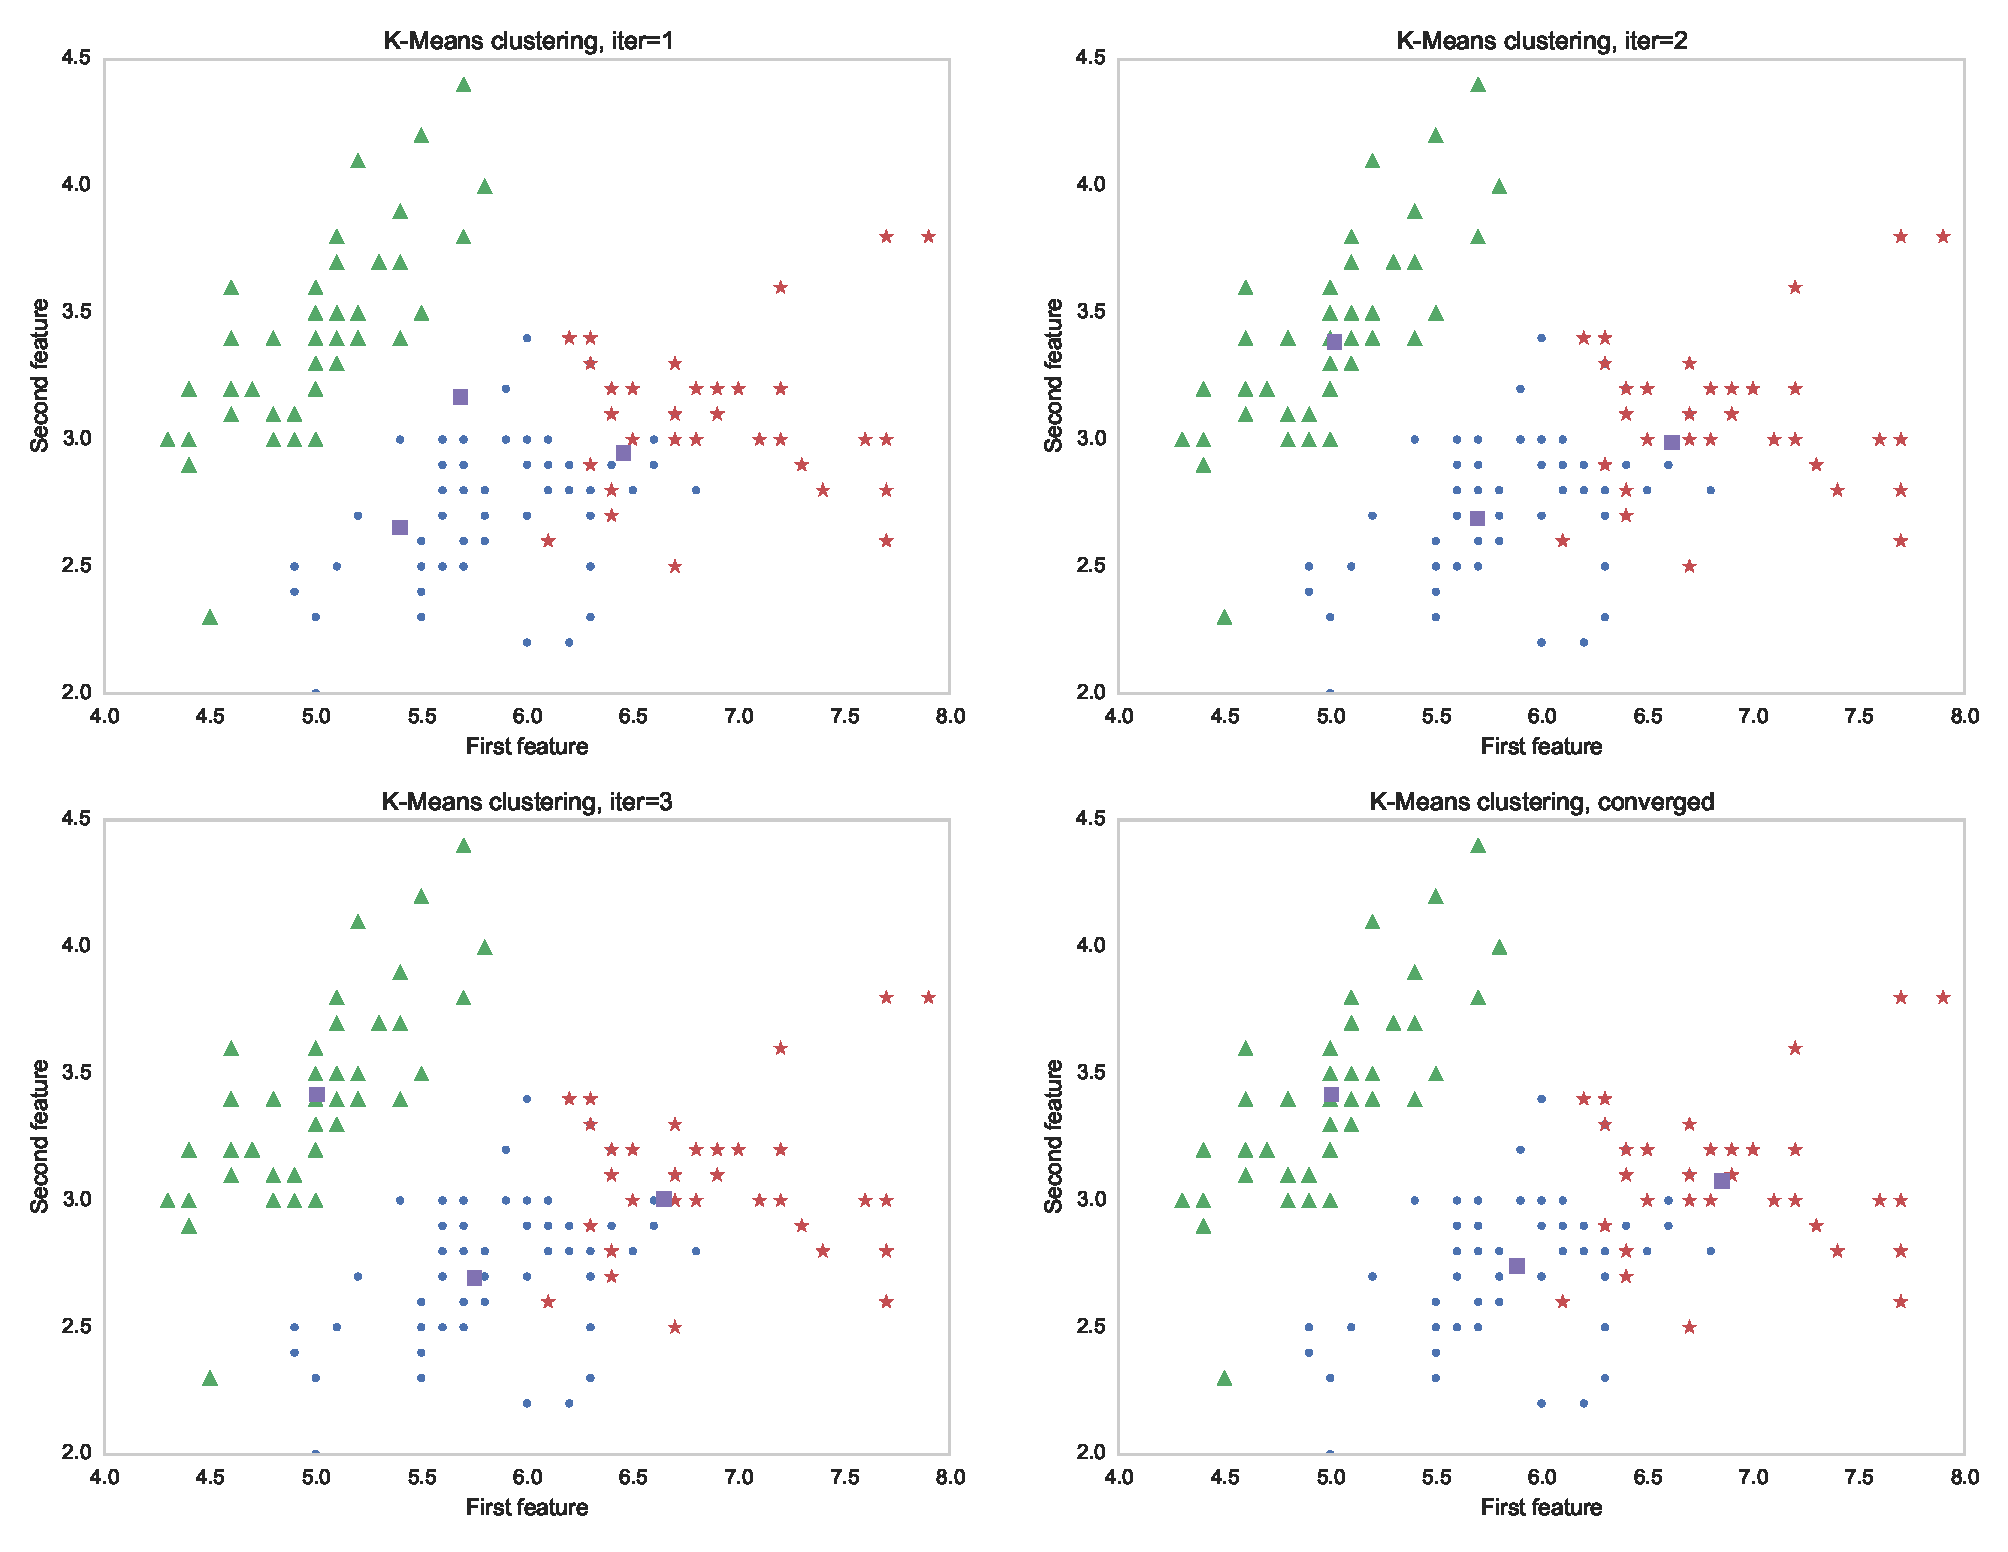
\includegraphics[width=\textwidth]{clustering/kmeans_progress}
    \caption{The output labels of the K-Means algorithm with the number of clusters (input parameter) set to 3. The different plots show the centroids (squares) evolution on each iteration. Between iteration 3 and the converged state 2 more iterations were executed.}
    \label{fig:intro kmeans}
\end{figure}

Even with the correct number of clusters, the clustering results do not match $100\%$ the natural clusters.
The accuracy relative to the natural clusters of Fig. \ref{fig:intro natural} is $88\%$ as measured by the Consistency Index (CI) \cite{Fred2001}.
In this example, the problem is the two overlapping clusters.
It is hard for an algorithm to discriminate between two clusters when they have similar patterns.
When no prior information about the dataset is given, the number of clusters can be hard to discover.
This is why, when available, a domain expert may provide valuable insight on tuning the initialization parameters.
% Others approaches, not addressed in this thesis, include the area of constrained clustering.

\section{Single-Link}
\label{sec:sl}

Single-Link \cite{sneath1962numerical} is one of the most popular hierarchical agglomerative clustering (HAC) algorithms.
HAC algorithms operate over a pair-wise dissimilarity matrix and outputs a dendrogram (e.g. Fig \ref{fig:sl dendrogram}).
The main steps of an agglomerative hierarchical clustering algorithm are the following \cite{Jain1999}:
\begin{enumerate}
    \item Create a pair-wise dissimilarity matrix of all patterns, where each pattern is a distinct cluster singleton;

    \item Find the closest clusters, merge them and update the matrix to reflect this change. The rows and columns of the two merged clusters are deleted and a new row and column are created to store the new cluster.% whose dissimilarities to other clusters will be the minimum of either the merging clusters.

    \item Stop if all patterns belong to a single cluster, otherwise continue to step 2.
\end{enumerate}

The algorithm stops when $n-1$ merges have been performed, which is when all patterns have been connected in the same cluster.
Just like in the K-Means algorithm, different similarity measures can be used for the distances.

%different linkages
The proximity between clusters in the second step is distinguishes between the different HAC linkage algorithms, such as Single-Link , Average-Link, Complete-Link, among others.
In Single-Link (SL), the proximity between any two clusters is the the dissimilarity between their closest patterns.
On the other hand, in Complete-Link, it is the proximity between their most distant patterns and, in Average-Link, is the proximity between the average point of each cluster.
In SL, because the algorithm connects first clusters that are more similar, it naturally gives more importance to regions of higher density \cite{Aggarwal2014}.

% naive & SLINK
The total time complexity of a naive implementation is $O(n^3)$ since it performs a $O(n^2)$ search in step two and it does it $n-1$ times.
Over time, more efficient implementations have been proposed, such as SLINK \cite{Sibson1973}.
SLINK needs no working copy of $O(n^2)$ the pair-wise similarity matrix (if the original can be modified), has a working memory of $O(n^2)$ and time complexity of $O(n^2)$.
This increase in performance comes from the observation that the $O(n^2)$ search can be transformed in a $O(n)$ search at the expense of keeping two arrays of length $n$ that will store the most similar cluster for each pattern and the corresponding similarity measure.
This way, to find the two closest clusters, the algorithm will not search the entire similarity matrix, but only the new similarity array since this array keeps the closest cluster of each cluster.
Naturally these arrays must be updated upon a cluster merge.

% SL from MST
An interesting property of the SL algorithm is its equivalence with a Minimum Spanning Tree (MST), an observation first made by \cite{Gower1969}.
In graph theory, a MST is a tree that connects all vertices together while minimizing the sum of all the distance between them.
An example of a graph and its corresponding MST can be seen in Fig. \ref{fig:mst example}.
In this context, the edges of the MST are the distances between the patterns and the vertices are the patterns themselves.
A MST contains all the information necessary to build a Single-Link dendrogram.
To walk down through the levels of the dendrogram from the MST, one cuts the least similar edges.
Furthermore, this approach can be used to apply Single-Link clustering to graphs-encoded problems in a straight-forward way.
Furthermore, the performance properties of this method are roughly the same as SLINK  \cite{Mullner2011}.

The true advantage of using an MST based approach comes when the number of edges (similarities) $m$ of the MST is less than $\frac{n(n-1)}{2}$, where $n$ is the number of nodes (patterns) \cite{starck2007astronomical}.
This is because SLINK works over a inter pattern similarity matrix, meaning that the similarity between every pair of patterns must be explicitly represented.
The minimum number of similarities is $\frac{n(n-1)}{2}$, which is equivalent to the upper or lower half triangular matrices of the similarity matrix.
The MST, on the other hand, works over a graph that may or may not have edges between every pair of nodes.
Fast MST algorithms have a time complexity of $O(m log n)$, which is an improvement over $O(n^2)$ when $m << \frac{n(n-1)}{2}$.


\begin{figure}[!ht]
    \centering
    \begin{subfigure}[b]{0.3\textwidth}
        \centering
        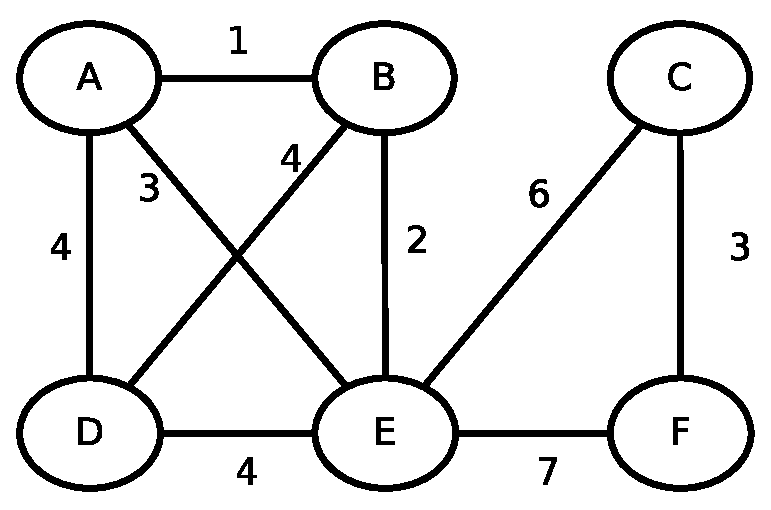
\includegraphics[width=\textwidth]{clustering/mst_graph}
        \caption{Example of a graph.}
        \label{fig:graph}
    \end{subfigure}
    %\hfill
    \hspace{30pt}
    \begin{subfigure}[b]{0.3\textwidth}
        \centering
        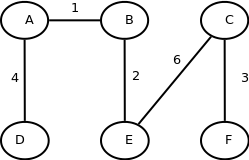
\includegraphics[width=\textwidth]{clustering/mst_mst}
        \caption{MST of the graph to the left.}
        \label{fig:graph mst}
    \end{subfigure}

    \caption{The above figures show an example of a graph (left) and its corresponding Minimum Spanning Tree (right). The circles are vertices and the edges are the lines linking the vertices.}
    \label{fig:mst example}
\end{figure}

An example of a Single-Link dendrogram and resulting cluster can be observed in Fig. \ref{fig:sl plots}.
The dendrogram in Fig. \ref{fig:sl dendrogram} has been truncated to 25 clusters in the bottom level for the sake of readability.
The clustering presented on Fig. \ref{fig:sl clustering} is the result of cutting the dendrogram such that only 3 clusters exist (the number of classes).
The accuracy, as measured by the CI, is of $58\%$.

\begin{figure}[!ht]
    \centering
    \begin{subfigure}[b]{0.45\textwidth}
        \centering
        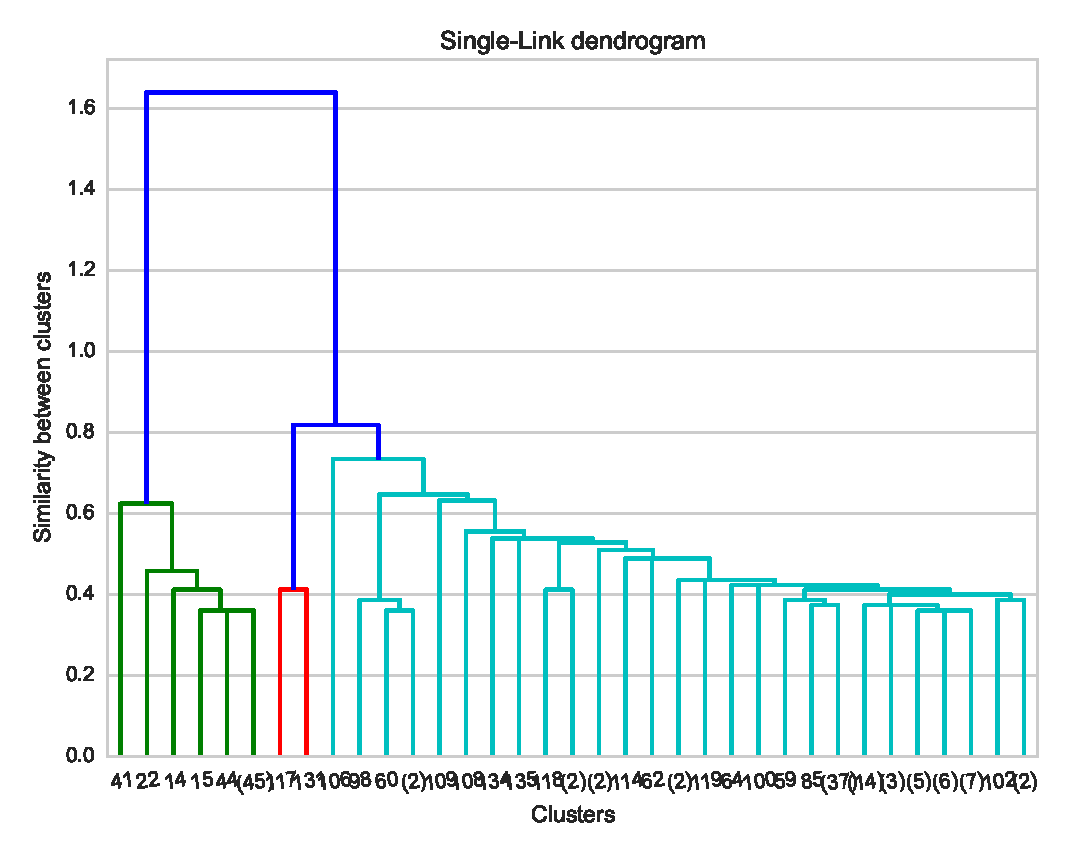
\includegraphics[width=\textwidth]{clustering/sl_dendrogram}
        \caption{Single-Link dendrogram truncated to 25 clusters in the bottom level.}
        \label{fig:sl dendrogram}
    \end{subfigure}
    %\hfill
    \begin{subfigure}[b]{0.45\textwidth}
        \centering
        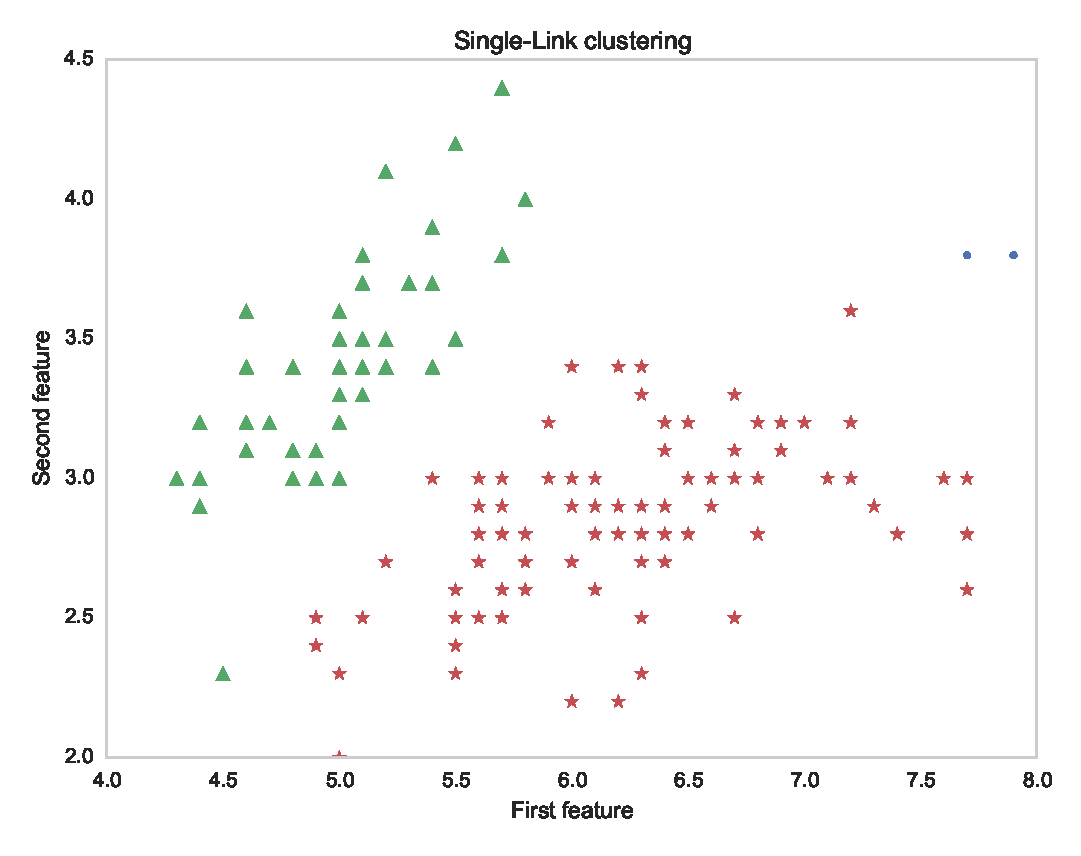
\includegraphics[width=\textwidth]{clustering/sl}
        \caption{Clustering with 3 clusters.}
        \label{fig:sl clustering}
    \end{subfigure}

    \caption{The above plots show the dendrogram and a possible clustering taken from a Single-Link run over the Iris data set. Fig. \ref{fig:sl clustering} was obtained by performing a cut on a level that would yield a partition of 3 clusters.}
    \label{fig:sl plots}
\end{figure}





% % % % % % % % % % % % % % % % % % % % % % % % % % % % % % % % % % % % % % % %
%
%                   EVIDENCE ACCUMULATION CLUSTERING
%
% % % % % % % % % % % % % % % % % % % % % % % % % % % % % % % % % % % % % % % %

\section{Ensemble Clustering}
\label{sec:ensemble}

The underlying idea behind ensemble clustering is to take a collection of partitions, a \emph{clustering ensemble}, and combine it into a single partition.
There are several motivations for ensemble clustering.
Data from real world problems appear in different configurations regarding shape, cardinality, dimensionality, sparsity, etc. 
Different clustering algorithms are appropriate for different data configurations, e.g. K-Means tends to group patterns in hyperspheres \cite{Jain1999} so it is more appropriate for data whose structure is formed by hypershere like clusters.
If the true structure of the data at hand is heterogeneous in its configuration, a single clustering algorithm might perform well for some part of the data while other performs better for some other part.
Since different algorithms can be used to produce the partitions in the ensemble, one can use a mix of algorithms to address different properties of the data such that the combination is more \textbf{robust} to noise and outliers \cite{topchy2004mixture} and the final clustering has a \textbf{better quality} \cite{Aggarwal2014}.
Ensemble clustering can also be particularly useful in situations where one does not have direct access to all the features of a given data set but can have access to partitions from different subsets and later combining with an ensemble algorithm.
Furthermore, the generation of the clustering ensemble can be \textbf{parallelized and distributed} since each partition is independent from every other partition.

A clustering ensemble, according to \cite{Fred2005}, can be produced from (1) different data representations, e.g. choice of preprocessing, feature selection and extraction, sampling; or (2) different partitions of the data, e.g. output of different algorithms, varying the initialization parameters on the same algorithm.

% different approaches to ensemble clustering
Ensemble clustering algorithms can take three main distinct approaches \cite{Aggarwal2014}: based on pair-wise similarities, probabilistic or direct.
EAC \cite{Fred2005} and CSPA \cite{Strehl2002} are examples of pair-wise similarity based approach, where the algorithms use a co-associations matrix.
The MMCE \cite{topchy2004mixture} and BCE \cite{wang2011bayesian} are examples of a probabilistic approach.
This approach will be further clarified when the EAC algorithm is explained.
HGPA \cite{Strehl2002}, MCLA \cite{Strehl2002} and bagging \cite{Dudoit2003} are examples of a direct approach to combining the ensemble clusterings, where the algorithms work directly with the labels without creating a co-association matrix.
A detailed and thorough review of the similarity measures that can be used on with clustering ensembles and the state of the art algorithms can be consulted in \cite{Aggarwal2014}.

% Many cluster ensemble algorithms exist, e.g. Bipartite \cite{Hore2009}, Metis Merger \cite{Hore2009}, CSPA \cite{Strehl2002}, HGPA \cite{Strehl2002}, MCLA \cite{Strehl2002} and EAC \cite{Fred2002}.

\section{Evidence Accumulation Clustering}
\label{sec:eac}

\subsection{Overview}

The goal of EAC is to find an optimal partition $P^*$ containing $k^*$ clusters, from the clustering ensemble $\mathbb{P}$. The optimal partition should have the following properties \cite{Fred2005}:

\begin{itemize}
    \item \textbf{Consistency} with the clustering ensemble;
    \item \textbf{Robustness} to small variations in the ensemble; and,
    \item \textbf{Goodness} of fit with ground truth information, when available.
\end{itemize}

\emph{Ground truth} is the true labels of each sample of the dataset, when such exists, and is used for validation purposes.
Since EAC is an unsupervised method, this typically will not be available.
EAC makes no assumption on the number of clusters in each data partition.
Its approach is divided in 3 steps:

\begin{enumerate}
\item \textbf{Production} of a clustering ensemble $\mathbb{P}$ (the evidence);
\item \textbf{Combination} of the ensemble into a co-association matrix;
\item \textbf{Recovery} of the natural clusters of the data.
\end{enumerate}

% introduce the creation of the ensemble
In the first step, a clustering ensemble is produced.
Within the context of EAC, it is of interest to have variety in the ensemble with the intention to better capture the underlying structure of the data.
One such parameter to measure that variety is the number of clusters in the partitions of the ensemble.
Typically, the number of clusters in each partition is drawn from an interval $[K_{min}, K_{max}]$ with uniform probability.
This influences other properties of other parts of the algorithm such as the sparsity of the co-association matrix as will become clearer in future chapters.
Reviewing the literature \cite{Fred2002,Fred2005,Lourenco2007,LourencoECG2009}, it is clear the ensemble is usually produced by random initialization of K-Means (specifying only the number of centroids within the above interval).
Still, other clustering algorithms have been used for the production of the ensemble \cite{Duarte2005} such as Single-Link, Average-Link and CLARANS.

The ensemble of partitions is combined in the second step, where a non-linear transformation turns the ensemble into a co-association matrix \cite{Fred2005}, i.e. a matrix $\mathcal{C}$ where each of its elements $n_{ij}$ is the association value between the pattern pair $(i,j)$.
The association between any pair of patterns is given by the number of times those two patterns appear clustered together in any cluster of any partition of the ensemble, i.e. the number of co-occurrences in the same cluster.
The rationale is that pairs that are frequently clustered together are more likely to be representative of a true link between the patterns \cite{Fred2002}, revealing the underlying structure of the data.
In other words, a high association $n_{ij}$ means it is more likely that patterns $i$ and $j$ belong to the same class.
The construction of the co-association matrix is at the very core of this method.

The co-association matrix itself is not the output of EAC.
Instead, it is used as input to other methods to obtain the final partition.
The co-association between any two patterns can be interpreted as a similarity measure.
Thus, since this matrix is a similarity matrix it's appropriate to use algorithms that take this type of matrices as input, e.g. K-Medoids or hierarchical algorithms such as Single-Link or Average-Link, to name a few.
Typically, algorithms use a distance as the dissimilarity, which means that they minimize the distance to obtain the highest similarity between objects.
However, a low value on the co-association matrix translates in a low similarity between a pair of objects, which means that the co-association matrix requires prior transformation for accurate clustering results, e.g. replace every similarity value $n_{ij}$ between every pair of object $(i,j)$ by $max \{ \mathcal{C} \} - n_{ij}$.

Although any algorithm can be used, the final clustering is usually done using SL or AL.
Each of this algorithms will take as input the transformed co-association matrix as the dissimilarity matrix.
Furthermore, not knowing the "natural" number of clusters one can use the lifetime criteria, i.e. the number of clusters $k$ should be such that it maximizes the cost of cutting the dendrogram from $k-1$ clusters to $k$.
Further details on the lifetime strategy for picking the number of clusters falls outside the scope of this work and are presented in \cite{Fred2005}.

% paragraph on weighted EAC: Weighting Cluster Ensembles in Evidence Accumulation Clustering
Related work to EAC has been developed.
The Weighted EAC (WEAC) algorithm \cite{Duarte2005} and a study on the sparsity of the co-association matrix \cite{Lourenco2010} should be mentioned.
The latter is discussed in more depth in chapter \ref{chapter:stateofart}.
The former introduces the novelty of having weights associated to each partition such that good quality partitions are more relevant than their counterparts.
These weights are based on internal validity measures.
Weighing the partitions in terms of quality has shown to improve the original algorithm, accuracy wise.

\subsection{Examples of applications}

EAC has been used with success in several areas. Some of its applications are:
\begin{itemize}
    \item in the field of bioinformatics it was used for the automatic identification of chronic lymphocyt leukemia \cite{Qian2010};
    \item also in bioinformatics it was used for the unsupervised analysis of ECG-based biometric database to highlight natural groups and gain further insight \cite{LourencoECG2009};
    \item in computer vision it was used as a solution to the problem of clustering of contour images (from hardware tools) \cite{Lourenco2007}.
\end{itemize}

% \subsection{Advantages and Disadvantages}
% %#REVIEW advantages and disadvantages of EAC

% An advantage of EAC is that it takes no input parameters such as the number of output clusters.
% Furthermore, it provides good accuracy on datasets with hard shapes \cite{Fred2005}.
% On the other hand, a big disadvantage is space complexity of the evidence combination step.
% In this step, when using the standard EAC, a co-association matrix is build, resulting in a complexity of $O(N^2)$.
% This translates in an almost prohibitive use of this method for bigger datasets.
